\documentclass[11pt]{article}

\usepackage[utf8]{inputenc}
\usepackage[T1]{fontenc}
\usepackage{lmodern}
\usepackage[margin=1in]{geometry}
\usepackage{amsmath,amssymb}
\usepackage{booktabs}
\usepackage{siunitx}
\usepackage{xcolor}
\usepackage{pgfplots}
\pgfplotsset{compat=1.17}
\usepackage[colorlinks=true,linkcolor=blue!50!black,urlcolor=blue!50!black]{hyperref}

\newcommand{\kbar}{\overline{\kappa}}
\newcommand{\um}{\si{\micro\meter}}
\newcommand{\uminv}{\si{\per\micro\meter}}
\newcommand{\code}[1]{\texttt{#1}}

\title{\textbf{Scale-Consistent Mean Curvature of\\ Osteon Formation-Front Contours}}
\author{OPALSx --- osteon profile and level-set analysis}
\date{\today}

\begin{document}
\maketitle

\begin{abstract}
The per-osteocyte curvature pipeline measures the curvature of a 2-D
formation-front contour over a fixed \emph{physical} arc length
$k_{\text{scale}}$ (\code{k\_scale\_um}). We observed that the reported
\emph{contour-mean} curvature varies strongly with $k_{\text{scale}}$ for
late-forming (small, inner) contours, while being stable for early (large) ones.
This note shows that the cause is a systematic bias of the local
parabola-fitting estimator whose relative size grows as
$(k_{\text{scale}}/L)^2$, where $L$ is the contour perimeter. The remedy is to
treat the contour mean as a \emph{global} quantity rather than averaging
scale-dependent local estimates. We give two window-free estimators that are
exactly independent of $k_{\text{scale}}$ and agree with the small-window limit of
the local estimate: the \emph{turning fit} $\kbar=2\pi/L$ (from the total turning,
Hopf's \emph{Umlaufsatz}) and the \emph{circle fit} $\kbar=1/R$ (a circle fitted
about the contour centroid). Both are implemented behind a single
\code{method} choice (\code{:ALF}/\code{:CCF}/\code{:CTF}, default
\code{:CCF}).
\end{abstract}

\section{Setup and notation}
\label{sec:setup}

At an osteocyte's formation time $t$ the level-set field
$\phi(t) = (1-t)\,S_{\text{out}} - t\,S_{\text{in}}$ is built (and Gaussian
smoothed) on the osteocyte's slice, and its zero contour
$\mathcal{C} = \{(x,y) : \phi = 0\}$ is extracted as a closed polygon with
vertices $P_1,\dots,P_N$ (with $P_{N+1}=P_1$), in physical units (\um).

For a smooth plane curve the \emph{signed curvature} is
\begin{equation}
  \kappa \;=\; \frac{x'\,y'' - y'\,x''}{\bigl(x'^2+y'^2\bigr)^{3/2}},
  \label{eq:kappa-def}
\end{equation}
and, for a graph $y=f(x)$,
\begin{equation}
  \kappa \;=\; \frac{f''}{\bigl(1+f'^2\bigr)^{3/2}}.
  \label{eq:kappa-graph}
\end{equation}

\paragraph{Local estimator (\code{compute\_2D\_curvature}).}
At each vertex $P_i$ the contour is translated to the origin and rotated so the
local tangent lies along the $x$-axis. A least-squares parabola
$y = a x^2 + b x + c$ is fitted to the vertices lying within an arc-length window
of total length $k_{\text{scale}}$ (i.e.\ $\pm h$, $h = k_{\text{scale}}/2$, on
each side). At the central point $x=0$ one has $f'(0)=b$, $f''(0)=2a$, so by
\eqref{eq:kappa-graph}
\begin{equation}
  \widehat{\kappa}_i \;=\; \frac{2a}{\bigl(1+b^2\bigr)^{3/2}}.
  \label{eq:kappa-est}
\end{equation}
The window $k_{\text{scale}}$ fixes the \emph{physical scale} at which curvature
is measured, so the same scale is used on contours of very different size.

\paragraph{Contour mean (as previously computed).}
The diagnostics reported the contour mean as the unweighted vertex average
\begin{equation}
  \langle\kappa\rangle \;=\; \frac{1}{N}\sum_{i=1}^{N}\widehat{\kappa}_i .
  \label{eq:mean-old}
\end{equation}

\section{The observed problem}
\label{sec:problem}

Sweeping $k_{\text{scale}}$ over $[10,150]\,\um$ on a single dataset
(\code{FM40-2-S2}) gives an early/large contour whose mean is nearly constant,
but a late/small contour whose mean inflates by more than a factor of two before
collapsing (Table~\ref{tab:summary}, Figure~\ref{fig:sweep}).

\begin{table}[h]
  \centering
  \begin{tabular}{rccccc}
    \toprule
    idx & $t$ & $L\ [\um]$ & $2\pi/L\ [\uminv]$ & $\langle\kappa\rangle$ mean $[\uminv]$ & CV over $k$ \\
    \midrule
     3 & 0.05 & 1009.9 & 0.00622 & 0.00631 & \phantom{0}2.8\,\% \\
    20 & 0.32 & \phantom{0}733.9 & 0.00856 & 0.00889 & \phantom{0}2.6\,\% \\
    37 & 0.92 & \phantom{0}179.3 & 0.03503 & 0.05436 & 28.3\,\% \\
    \bottomrule
  \end{tabular}
  \caption{Mean curvature of three contours, swept over
    $k_{\text{scale}}\in[10,150]\,\um$ in steps of $10\,\um$. The coefficient of
    variation (CV $=$ std$/$mean across the sweep) is small for the large
    contours but explodes for the small late contour. $2\pi/L$ is the
    scale-invariant value derived in Section~\ref{sec:turning}.}
  \label{tab:summary}
\end{table}

\begin{figure}[h]
  \centering
  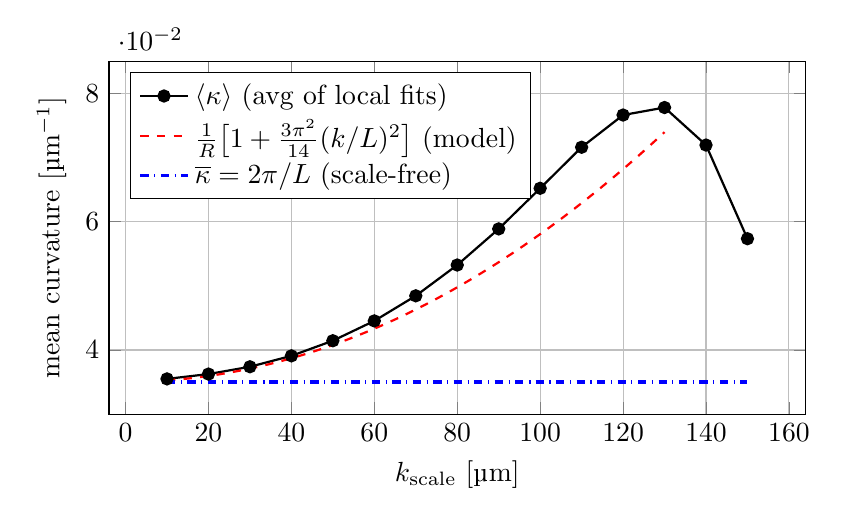
\begin{tikzpicture}
    \begin{axis}[
        width=0.86\textwidth, height=0.5\textwidth,
        xlabel={$k_{\text{scale}}\ [\um]$},
        ylabel={mean curvature $[\uminv]$},
        legend pos=north west, legend cell align=left,
        grid=both, ymin=0.03, ymax=0.085,
      ]
      % empirical unweighted mean for the late contour (idx 37, L = 179.3)
      \addplot[mark=*,thick,black] coordinates {
        (10,0.03550)(20,0.03625)(30,0.03739)(40,0.03909)(50,0.04145)
        (60,0.04454)(70,0.04845)(80,0.05325)(90,0.05888)(100,0.06521)
        (110,0.07161)(120,0.07663)(130,0.07780)(140,0.07195)(150,0.05735)};
      \addlegendentry{$\langle\kappa\rangle$ (avg of local fits)}
      % leading-order (k/L)^2 model
      \addplot[red,dashed,thick,domain=10:130,samples=40] {0.03503*(1+2.114*(x/179.3)^2)};
      \addlegendentry{$\tfrac{1}{R}\bigl[1+\tfrac{3\pi^2}{14}(k/L)^2\bigr]$ (model)}
      % scale-free turning mean
      \addplot[blue,dash dot,very thick,domain=10:150] {0.03503};
      \addlegendentry{$\kbar=2\pi/L$ (scale-free)}
    \end{axis}
  \end{tikzpicture}
  \caption{Late contour (idx 37, $L=179.3\,\um$). The averaged local estimate
    (black) departs from the true mean $2\pi/L$ (blue) as the window grows,
    tracking the leading-order $(k/L)^2$ bias (red) until the window becomes a
    large fraction of the perimeter and the fit degenerates entirely.}
  \label{fig:sweep}
\end{figure}

Two facts narrow down the cause:
\begin{enumerate}
  \item At small $k_{\text{scale}}$ the mean converges to $2\pi/L$
    ($0.0355 \to 0.0350$ for idx~37); the inflation appears only as the window
    grows.
  \item Replacing the unweighted average \eqref{eq:mean-old} with the
    arc-length-weighted average
    $\sum_i \widehat{\kappa}_i\,\Delta s_i / \sum_i \Delta s_i$ changes nothing
    (CV stays $28\,\%$): marching-squares vertices are near-uniformly spaced, so
    the two averages coincide. The problem is therefore in the per-vertex
    estimates $\widehat{\kappa}_i$ themselves, not in how they are averaged.
\end{enumerate}

\section{Why the local estimator is scale-dependent}
\label{sec:bias}

Consider the cleanest case: $\mathcal{C}$ is a circle of radius $R$, so the true
curvature is $1/R$ everywhere. In the tangent frame at the fitting point the
circle is the graph
\begin{equation}
  f(x) \;=\; R-\sqrt{R^2-x^2}
        \;=\; \frac{x^2}{2R} + \frac{x^4}{8R^3} + \frac{x^6}{16R^5} + \cdots
  \label{eq:circle-graph}
\end{equation}
The estimator \eqref{eq:kappa-est} fits only a quadratic, so the quartic and
higher terms in \eqref{eq:circle-graph} leak into the fitted coefficient $a$ and
bias it. By symmetry $b=0$, and the least-squares estimate of $a$ is obtained by
projecting $f$ onto $\{1,x^2\}$ over the fitting interval $[-X,X]$, where
$X = R\sin\Phi$ is the half-width in $x$ and $\Phi$ the half-arc subtended at the
centre.

Regressing $x^4$ onto $\{1,x^2\}$ over $[-X,X]$ (uniform measure) gives the
$x^2$-coefficient
\begin{equation}
  q \;=\; \frac{M_0 M_6 - M_2 M_4}{M_0 M_4 - M_2^2}
    \;=\; \frac{\tfrac{4}{7}-\tfrac{4}{15}}{\tfrac{4}{5}-\tfrac{4}{9}}\,X^2
    \;=\; \frac{6}{7}\,X^2,
  \qquad M_{2k}=\int_{-X}^{X}\! x^{2k}\,dx,
\end{equation}
so to leading order
\begin{equation}
  \widehat{a} \;=\; \frac{1}{2R} + \frac{1}{8R^3}\cdot\frac{6}{7}X^2 + \cdots,
  \qquad
  \widehat{\kappa} \;=\; 2\widehat{a}
  \;=\; \frac{1}{R}\left[\,1 + \frac{3}{14}\Bigl(\frac{X}{R}\Bigr)^2 + \cdots\right].
  \label{eq:bias-1}
\end{equation}
The bias is positive: a parabola fitted over a wide arc must reach the far,
``flattening'' points of the circle, which it can only do by curving more
sharply, so $\widehat{\kappa}>1/R$. (In the extreme $\Phi\to\pi/2$, the far point
is $(R,R)$ and a parabola through it has $aR^2=R$, i.e.\ $\widehat\kappa = 2/R$,
double the truth.)

\paragraph{Linking the window to the contour size.}
The half-window in arc length is $h=k_{\text{scale}}/2 = R\Phi$, so
$\Phi = k_{\text{scale}}/(2R)$. Writing the radius in terms of the perimeter via
the effective radius $R_{\text{eff}} = L/2\pi$ (exact for a circle, and the
natural size scale for a general convex contour, Section~\ref{sec:turning}),
\begin{equation}
  \Phi \;=\; \frac{k_{\text{scale}}}{2R_{\text{eff}}}
        \;=\; \pi\,\frac{k_{\text{scale}}}{L}.
\end{equation}
For modest windows $X/R\approx\Phi$, and \eqref{eq:bias-1} becomes a clean law in
the dimensionless ratio $k_{\text{scale}}/L$:
\begin{equation}
  \boxed{\;
  \frac{\widehat{\kappa}}{\kappa_{\text{true}}}
  \;\approx\; 1 + \frac{3}{14}\,\Phi^2
  \;=\; 1 + \frac{3\pi^2}{14}\Bigl(\frac{k_{\text{scale}}}{L}\Bigr)^2
  \;\approx\; 1 + 2.11\Bigl(\frac{k_{\text{scale}}}{L}\Bigr)^2 .
  \;}
  \label{eq:bias-law}
\end{equation}
This explains every feature of the data:
\begin{itemize}
  \item the bias is \emph{quadratic} in $k_{\text{scale}}/L$, hence negligible
    for large early contours ($k_{\text{scale}}/L\!\ll\!1$) and large for small
    late contours;
  \item for idx~37 at $k_{\text{scale}}=60\,\um$, $k_{\text{scale}}/L=0.33$ and
    \eqref{eq:bias-law} predicts $+24\,\%$ (observed $+27\,\%$; the remaining
    excess is the neglected $x^6$ and higher terms, which steepen the curve);
  \item once $k_{\text{scale}}\sim L$ the window wraps most of the contour, the
    fit is meaningless, and the curve in Figure~\ref{fig:sweep} turns over.
\end{itemize}

Crucially, the bias \eqref{eq:bias-law} is a property of \emph{each}
$\widehat{\kappa}_i$. No reweighting of the $\widehat{\kappa}_i$ can remove it ---
which is exactly why the arc-length-weighted average behaves identically to the
unweighted one.

\section{Two scale-invariant alternatives}
\label{sec:turning}

The mean curvature of a \emph{closed} contour need not be estimated locally at
all. We give two window-free estimators; both reduce to $1/R$ for a circle and
neither depends on $k_{\text{scale}}$.

\subsection{Contour turning fit (\texttt{:CTF})}
\label{sec:ctf}

For a positively oriented, simple, closed $C^2$ curve, the theorem of turning
tangents (Hopf's \emph{Umlaufsatz}) states
\begin{equation}
  \oint_{\mathcal{C}} \kappa \, ds \;=\; 2\pi\, n,
  \label{eq:umlauf}
\end{equation}
where $n$ is the turning (rotation) number; $n=1$ for a simple convex contour.
The \emph{arc-length-weighted} mean curvature is therefore independent of any
measurement window:
\begin{equation}
  \boxed{\;
  \kbar_{\text{CTF}} \;=\; \frac{\oint_{\mathcal{C}}\kappa\,ds}{\oint_{\mathcal{C}} ds}
        \;=\; \frac{2\pi n}{L}
        \;=\; \frac{2\pi}{L}
        \;=\; \frac{1}{R_{\text{eff}}}
  \quad(\text{simple contour}).
  \;}
  \label{eq:kbar}
\end{equation}
This is the value $\langle\kappa\rangle$ converges to as $k_{\text{scale}}\to 0$
in Figure~\ref{fig:sweep}: from \eqref{eq:bias-law}, the arc-length integral of
the \emph{unbiased} curvature is $2\pi$, while at finite window the integral of
the inflated $\widehat\kappa$ exceeds $2\pi$, pushing the average above $2\pi/L$.
Discretely, for the polygon $P_1,\dots,P_N$ with edge vectors
$\mathbf{e}_i = P_{i+1}-P_i$, the integral \eqref{eq:umlauf} is a sum of exterior
(turning) angles,
\begin{equation}
  \theta_i \;=\; \operatorname{atan2}\!\bigl(\mathbf{e}_{i-1}\times\mathbf{e}_i,\;
                                            \mathbf{e}_{i-1}\cdot\mathbf{e}_i\bigr),
  \qquad
  \sum_{i=1}^{N}\theta_i \;=\; 2\pi n,
  \qquad
  \kbar_{\text{CTF}} \;=\; \frac{\sum_i \theta_i}{\sum_i \lvert\mathbf{e}_i\rvert},
  \label{eq:kbar-discrete}
\end{equation}
which holds exactly for any simple closed polygon regardless of vertex spacing
(implemented as \code{turning\_fit\_curvature}).

\subsection{Contour circle fit (\texttt{:CCF}, default)}
\label{sec:ccf}

Alternatively, fit a circle to all contour vertices with its centre fixed at the
centroid $\bar P = \tfrac1N\sum_i P_i$, and read the mean curvature as the inverse
of the fitted radius. With the centre fixed, the least-squares radius minimises
\begin{equation}
  E(R) \;=\; \sum_{i=1}^{N}\bigl(r_i - R\bigr)^2,
  \qquad r_i = \lVert P_i - \bar P\rVert,
\end{equation}
and, since $E'(R) = -2\sum_i (r_i - R) = 0$, has the closed form ``mean radial
distance'':
\begin{equation}
  \boxed{\;
  R \;=\; \frac1N\sum_{i=1}^{N}\lVert P_i - \bar P\rVert,
  \qquad
  \kbar_{\text{CCF}} \;=\; \frac1R .
  \;}
  \label{eq:kbar-circle}
\end{equation}
For a circle the $P_i$ are equidistant from the centre $=\bar P$, so $R$ is the
true radius and $\kbar_{\text{CCF}}=1/R$ exactly. Like the turning fit,
\eqref{eq:kbar-circle} uses no measurement window (implemented as
\code{circle\_fit\_curvature}).

\paragraph{How the two differ.} Both write $\kbar = 1/R_{\text{eff}}$ but use
different effective radii,
\begin{equation}
  R_{\text{eff}}^{\text{CTF}} = \frac{L}{2\pi}
  \quad(\text{perimeter radius}),
  \qquad
  R_{\text{eff}}^{\text{CCF}} = \frac1N\sum_i \lVert P_i - \bar P\rVert
  \quad(\text{radial-mean radius}).
\end{equation}
They coincide for a circle. For a wiggly boundary the perimeter radius is
sensitive to small-scale roughness (crenellation inflates $L$ and hence
$\kbar_{\text{CTF}}$), whereas the radial-mean radius averages such roughness out
but presumes the contour is reasonably centred and round. For the near-circular
osteon contours the two agree closely (Section~\ref{sec:verify}).

\section{Verification}
\label{sec:verify}

Both window-free estimators reproduce $1/R$ and agree with the reliable
small-window limit of the local estimator, with zero scale dependence:

\begin{center}
  \begin{tabular}{rccccc}
    \toprule
    idx & $t$ & turning $\tfrac{2\pi}{L}$ & circle $\tfrac1R$ & small-$k$ ($k{=}10$) & averaged $\langle\kappa\rangle$ CV \\
    \midrule
     3 & 0.05 & 0.00622 & 0.00649 & 0.00646 & \phantom{0}2.8\,\% \\
    20 & 0.32 & 0.00856 & 0.00884 & 0.00863 & \phantom{0}2.6\,\% \\
    37 & 0.92 & 0.03503 & 0.03510 & 0.03550 & 28.3\,\% \\
    \bottomrule
  \end{tabular}
\end{center}

The turning ($2\pi/L$) and circle ($1/R$) means agree with each other and with
the (reliable) small-window estimate to within a few percent on every contour,
while the windowed average drifts by up to $28\,\%$ on the small late contour. On
a perfect circle of radius $30\,\um$ all three methods return
$1/R = 0.0333\,\uminv$ (the average of local fits at $k_{\text{scale}}=20\,\um$
gives $0.0342$, the expected $\sim$$2\,\%$ window bias).

\section{Implementation and recommendations}
\label{sec:reco}

The three estimators are exposed through a single method choice,
\begin{center}
  \code{contour\_mean\_curvature(x, y; method=:CCF, arclen=nothing)},
\end{center}
with \code{method} one of:
\begin{itemize}
  \item \code{:ALF} --- \emph{average of local fits}, $\langle\kappa\rangle$
    \eqref{eq:mean-old}; scale-dependent, uses the window \code{arclen}
    ($=k_{\text{scale}}$);
  \item \code{:CCF} --- \emph{contour circle fit} \eqref{eq:kbar-circle};
    scale-free \textbf{(default)};
  \item \code{:CTF} --- \emph{contour turning fit} \eqref{eq:kbar-discrete};
    scale-free.
\end{itemize}
The same \code{mean\_method} keyword is threaded through
\code{compute\_curvature\_near\_osteocyte} (which returns
\code{mean\_available\_$\kappa$}) and \code{plot\_osteocyte\_contour}; both
default to \code{:CCF}.

\paragraph{Recommendations.}
\begin{itemize}
  \item \textbf{Report the contour mean with \code{:CCF} (default) or \code{:CTF}.}
    Both are exact for a circle, robust to sampling, and free of the
    $(k_{\text{scale}}/L)^2$ bias of \code{:ALF}.
  \item \textbf{Keep the windowed per-vertex estimator
    (\code{compute\_2D\_curvature}) for \emph{local} curvature} (e.g.\ at the
    osteocyte), where a fixed physical scale is the intent. To hold its bias below
    $\sim\!2\,\%$, choose $k_{\text{scale}}/L \lesssim 0.1$ for the
    \emph{smallest} contour of interest (from \eqref{eq:bias-law},
    $2.11\times0.1^2\approx0.02$).
  \item \textbf{Interpretational caveat.} Both window-free means are \emph{size}
    measures ($1/R_{\text{eff}}$): by \eqref{eq:umlauf} every simple closed
    contour has total turning $2\pi$ regardless of local concavities, so neither
    $\kbar_{\text{CTF}}$ nor $\kbar_{\text{CCF}}$ can distinguish convex- from
    concave-preferring embedding. That question is inherently \emph{local} and
    must be read from the per-vertex $\widehat{\kappa}_i$ (e.g.\ $\kappa$ at the
    osteocyte relative to $\kbar$), measured at an appropriately small
    $k_{\text{scale}}$.
\end{itemize}

\end{document}
